\documentclass[logo,reportComp]{thesis}
\usepackage[cpp,linenum]{mypackage}

\title{计算机网络实验报告}
\subtitle{实验五:文件传输实验(选做)}
\school{数据科学与计算机学院}
\author{陈鸿峥}
\classname{17大数据与人工智能}
\stunum{17341015}
\headercontext{计算机网络实验报告}

\begin{document}

\maketitle

\section{实验目的}
学习利用套接字传送文件。

\section{实验工具}
Telnet或SecureCRT

\section{实验环境}
本机为Ubuntu 18.04 (LTS) + gcc 7.3.0

\section{实验内容}
利用数据表示实验和Echo实验实现以下功能:
\begin{enumerate}
    \item 运行服务器端程序,输入接收文件的文件夹,然后等待客户端连接,并接收客户端发来的文件并保存,直到客户端关闭连接。有重名文件时,文件名增加序号保存。
    \item 客户端先连接服务器,每次输入一个文件名(包含路径)就传输它,直到输入\verb'exit'时退出并关闭套接字。
\end{enumerate}

\section{实验结果}
运行成功后,服务器截屏:
\begin{figure}[H]
\centering
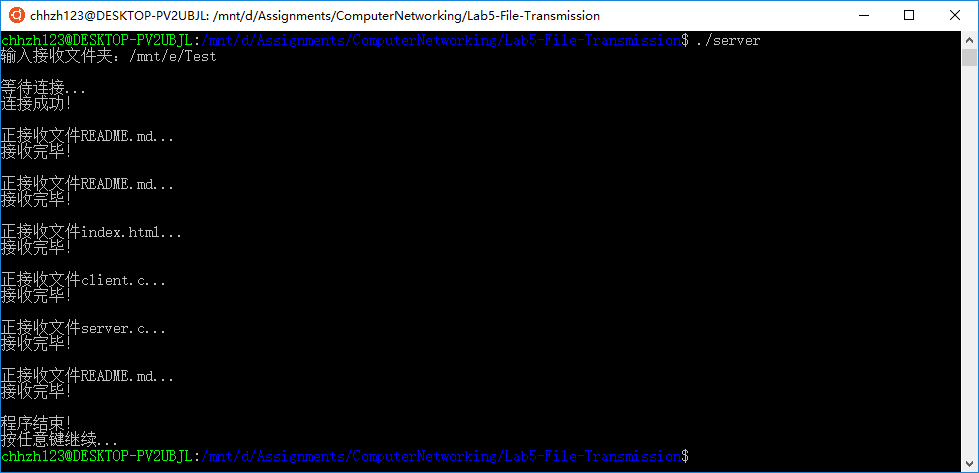
\includegraphics[width=0.8\linewidth]{fig/server.PNG}
\end{figure}

客户端运行截屏:
\begin{figure}[H]
\centering
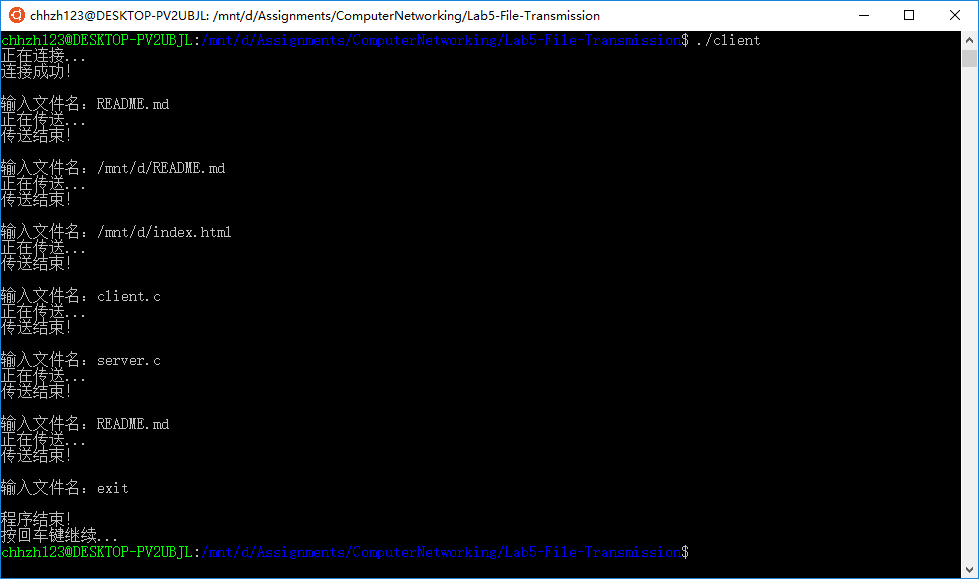
\includegraphics[width=0.8\linewidth]{fig/client.PNG}
\end{figure}

目标文件夹:
\begin{figure}[H]
\centering
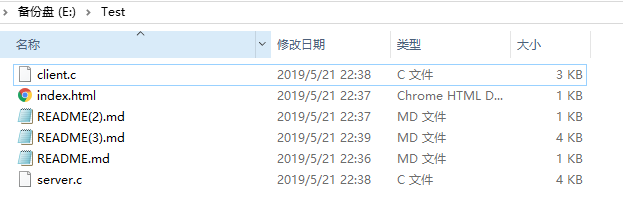
\includegraphics[width=0.8\linewidth]{fig/file.PNG}
\end{figure}

除了下面的服务器和客户端程序外,还自己写了\verb'Makefile'文件方便编译。

服务器程序:
\begin{lstlisting}
#include <sys/types.h>
#include <sys/socket.h>
#include <netinet/in.h>
#include <arpa/inet.h>
#include <stdio.h>
#include <stdlib.h>
#include <string.h>
#include <unistd.h>

#define BUF_LEN 100000

int main(int argc, char *argv[])
{
    struct  sockaddr_in fsin;               /* the from address of a client   */
    int     msock, ssock;                   /* master & slave sockets         */
    char    *service = "50500";
    char    buf[100];                       /* buffer for file name           */
    char    res[BUF_LEN];                   /* buffer for file context        */
    struct  sockaddr_in sin;                /* an Internet endpoint address   */
    int     alen;                           /* from-address length            */
    char    *pts;                           /* pointer to time string         */

    char path[100];
    printf("`输入接收文件夹:'");
    scanf("%s",path);

    printf("\n`等待连接'...\n");
    // create socket
    msock = socket(PF_INET, SOCK_STREAM, IPPROTO_TCP);

    memset(&sin,'\0', sizeof(sin));
    sin.sin_family = AF_INET;
    sin.sin_addr.s_addr = INADDR_ANY;
    sin.sin_port = htons((u_short)atoi(service));
    bind(msock, (struct sockaddr *)&sin, sizeof(sin));

    listen(msock, 5); // length-5 request queue
    alen = sizeof(struct sockaddr);
    ssock = accept(msock, (struct sockaddr *)&fsin, &alen);
    printf("`连接成功!'\n\n");

    while (1){
        memset(buf,sizeof(buf),0);
        memset(res,sizeof(res),0);
        char tmppath[100];
        strcpy(tmppath,path);

        // receive file name
        int cc = recv(ssock, buf, BUF_LEN, 0);
        if (cc <= 0) // client closed
            break;
        else if (cc > 0) {
            buf[cc] = '\0';

            printf("`正接收文件'%s...\n", buf);
            int cc = recv(ssock, res, BUF_LEN, 0);
            
            // test if file exists
            int cnt = 1;
            strcat(tmppath,"/"); // must in Linux!
            strcat(tmppath,buf);
            char file_name[100];
            while (1){
                strcpy(file_name,tmppath);
                if (cnt != 1) {
                    char* p = strchr(file_name,'.');
                    if (p != 0) { // not found
                        char suffix[10];
                        strcpy(suffix,p);
                        *p = '\0';
                        strcat(file_name,"(");
                        char numstr[10];
                        sprintf(numstr,"%d",cnt);
                        strcat(file_name,numstr);
                        strcat(file_name,")");
                        strcat(file_name,suffix);
                    } else {
                        strcat(file_name,"(");
                        char numstr[10];
                        sprintf(numstr,"%d",cnt);
                        strcat(file_name,numstr);
                        strcat(file_name,")");
                    }
                }
                if (access(file_name, F_OK ) == -1)
                    break;
                cnt++;
            }
            FILE* fout = fopen(file_name,"wb");
            fwrite(res,strlen(res),1,fout);
            fclose(fout);
            printf("`接收完毕!'\n\n");
        }
    }
    close(ssock);
    close(msock);
    printf("`程序结束!'\n`按任意键继续'...\n");
    getchar();
    return 0;
}
\end{lstlisting}

客户端程序:
\begin{lstlisting}
#include <sys/types.h>
#include <sys/socket.h>
#include <netinet/in.h>
#include <arpa/inet.h>
#include <stdio.h>
#include <unistd.h>
#include <stdlib.h>
#include <string.h>
#include <assert.h>

#define BUF_LEN 100000

int main(int argc, char *argv[])
{
    char    *host = "127.0.0.1";       /* server IP to connect         */
    char    *service = "50500";        /* server port to connect       */
    struct  sockaddr_in sin;           /* an Internet endpoint address */
    char    buf[100];                  /* buffer for file name         */
    char    res[BUF_LEN];              /* buffer for file context      */
    int     sock;                      /* socket descriptor            */
    int     cc;                        /* recv character count         */

    printf("`正在连接'...\n");

    // create socket
    sock = socket(PF_INET, SOCK_STREAM, IPPROTO_TCP);

    memset(&sin, 0, sizeof(sin));
    sin.sin_family = AF_INET;
    sin.sin_addr.s_addr = inet_addr(host);
    sin.sin_port = htons((u_short)atoi(service));
    int ret = connect(sock, (struct sockaddr *)&sin, sizeof(sin));
    printf("`连接成功!'\n\n");

    while (1){
        printf("`输入文件名:'");
        scanf("%s", buf);
        if (strcmp(buf,"exit") == 0)
            break;
        // split string
        char path[100], *file_name;
        strcpy(path,buf);
        char* str = buf;
        char* p = strsep(&str,"/"); // must in Linux!
        while (p != NULL)
        {
            file_name = p;
            p = strsep(&str,"/");
        }

        cc = send(sock, file_name, strlen(file_name), 0);
        assert(cc > 0);

        printf("`正在传送'...\n");
        FILE* fin = fopen(path,"rb");
        assert(fin != NULL);
        // get file size
        fseek(fin,0,SEEK_END);
        long size = ftell(fin);
        rewind(fin);

        fread(res,size,1,fin);
        cc = send(sock, res, strlen(res), 0);

        fclose(fin);
        printf("`传送结束!'\n\n");
    }

    close(sock);
    printf("\n`程序结束!'\n`按回车键继续'...\n");
    getchar();
    return 0;
}
\end{lstlisting}

\section{实验体会}
% 写出实验过程中遇到的问题,解决方法和自己的思考;并简述实验体会(如果有的话)。
本次实验使用第一第二次实验的代码,只需将用户交互界面修改一下即可。
同样注意文件命名的问题,第一次实现的时候采用C++进行字符串处理,现在改回使用C语言,发现也没有想象中的那么麻烦。

\end{document}
% http://www.cplusplus.com/doc/tutorial/files/

% 【交实验报告】
% (1) 每位同学单独完成本实验内容并填写实验报告。
% (2) 上交网址:http://172.18.187.9/netdisk/default.aspx?vm=17net  实验上交/编程实验
% (3) 截止日期(不迟于):2019年6月15日 23:00 (周六)。
% 上传文件:学号_姓名_文件传输实验.doc   (不要用PDF文件)
%          学号_姓名_文件传输实验.rar 